\section{Ảnh hưởng của giảm chiều bằng PCA}
\label{sec:6_3}
So sánh ba cấu hình trên cùng các fold, với PCA chỉ fit từ phần train của từng fold:
\begin{table}[htbp]
\centering\scriptsize
\caption{So sánh không PCA và hai ngưỡng giữ phương sai}\label{tab:cv-pca}
\begin{tabular}{lrrrr}
\toprule
Cấu hình & F1 CV & SD & Precision & Recall \\
\midrule
lr\_c1 & 0,6557 & 0,0078 & 0,7315 & 0,5943 \\
lr\_pca90 & 0,6427 & 0,0057 & 0,7322 & 0,5728 \\
lr\_pca95 & 0,6476 & 0,0033 & 0,7301 & 0,5819 \\
\bottomrule
\end{tabular}
\end{table}
\begin{figure}[htbp]
\centering
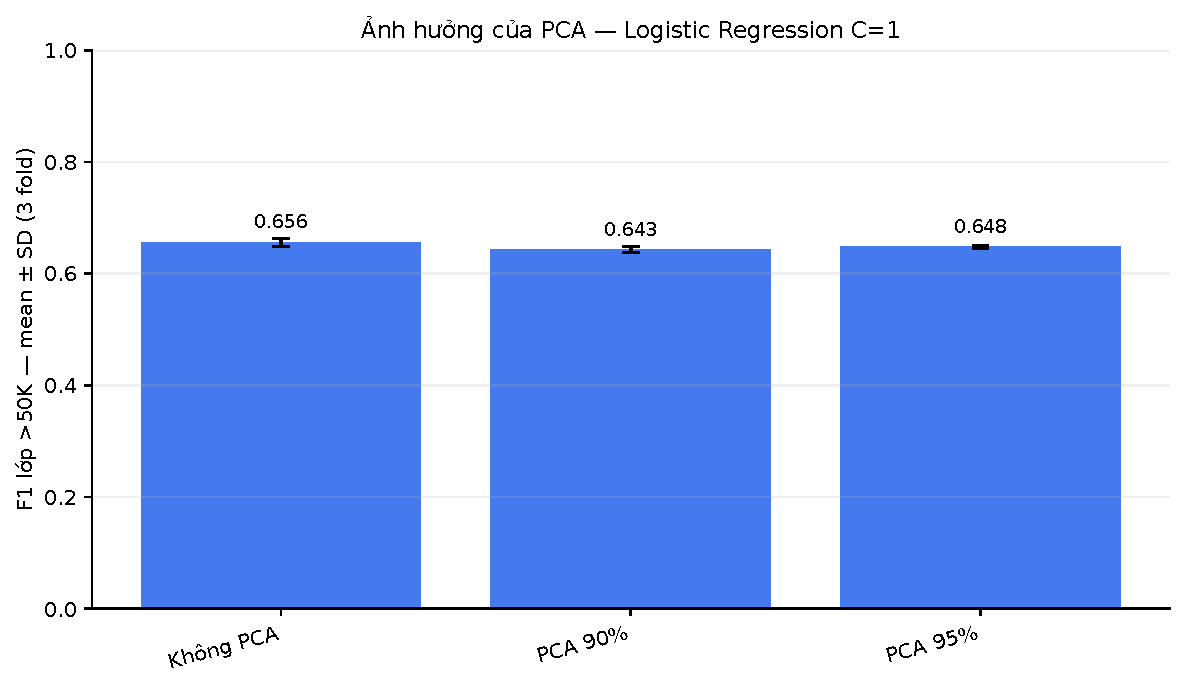
\includegraphics[width=.95\textwidth]{Images/chapter_6/6_3/cv_pca.pdf}
\caption{F1 CV của Logistic Regression C=1 khi thay lựa chọn PCA}
\label{fig:cv-pca}
\end{figure}
PCA giảm số chiều nhưng tối ưu phương sai của đầu vào, không sử dụng nhãn để chọn hướng. Vì vậy, giảm chiều có thể làm mất thông tin hữu ích cho phân loại. Các kết quả này được dùng để nhận xét riêng thí nghiệm PCA trên Logistic Regression; không suy rộng tác động sang Random Forest hoặc MLP chưa chạy với PCA.

% BEGIN REVIEW ANALYSIS
Ở bộ đặc trưng fit trên toàn bộ train, số chiều giảm từ 105 xuống 22 với PCA 90\% và 31 với PCA 95\%, tương ứng giảm 79,05\% và 70,48\%. Đây là kích thước của các tệp NumPy xuất từ toàn bộ train; từng fold CV vẫn tự fit encoder/PCA và có thể có số chiều khác. F1 CV thay đổi -1,30 và -0,82 điểm phần trăm so với không PCA. Như vậy, trong thí nghiệm này, tiết kiệm chiều đi kèm giảm F1; không chọn PCA chỉ vì giữ được một tỷ lệ phương sai cao.
% END REVIEW ANALYSIS
